\part{Construction du modèle}
    \chapter{Les principes généraux}
        \section{Contenu du texte d'une liste d'ingrédients}

        En général, chaque ingrédient sera présent une seule fois dans la liste (cf. section \mref{listes_ingredients})

        Le calcul d'embeddings via des modèles tels que SVD ou Word2Vec fait peu de sens.
        \newline
        \newline
        \emphbox{l'extraction des textes se fait au format \emph{Bag Of Words}, sans utiliser de notion d'IDF. L'utilsation de TF semble églament ne pas amener de valeur à priori.}

        \section{Limitation à l'identification des listes d'ingrédients}

        On est sur une taxonomie d'informations limitée dans les fiches techniques.

        On pourrait envisager de classifier l'ensemble des textes présents dans les fiches techniques.

        Mais l'absence de données étiquetées rend cette tâche impossible. La charge d'étiquetage d'un nombre représentatif de blocs de texte de fiches techniques est trop importante pour être mise en oeuvre dans le cadre de ce projet.

        \section{Conversion de documents en texte}
        
        dire ici qu'on utilise principalement pdfminer vs. d'autres outils d'OCR.

        De plus, on partira dans un premier temps sur une transformation basique d'un document en texte, sans passer par une analyse de la localisation des textes sur le document (cf. les difficultés présentées dans la section \mref{formats_spatialisation}).
            
    \chapter{Construction d'un modèle simple \og ouvert \fg}
        
    Le fonctionnement global de ce premier modèle (présenté à la \reffig{fig:open_model}) ne respecte pas les principes du Machine Learning.
    Il permet juste d'éprouver la méthode préssentie, ainsi que de se faire une idée de l'efficacité d'un modèle de ce type.
    En effet, même si on utilise des briques d'extraction de features depuis des textes, il manque une partie de mesure de la performance, indispensable pour pouvoir évaluer et améliorer la pertinence du modèle.
    On peut toutefois tout de même effectuer un train/test split, afin d'éviter de surestimer la valeur des résultats.    
    Le code est présenté en annexe (ref à mettre), il utilise les classes IngredientExtractor et PIMIngredientExtractor.
    Il n'utilise pas les données étiquetées manuellement (présentées à la section \mref{manually_labelled_data}).

    \begin{figure}[htbp]
        \begin{center}
        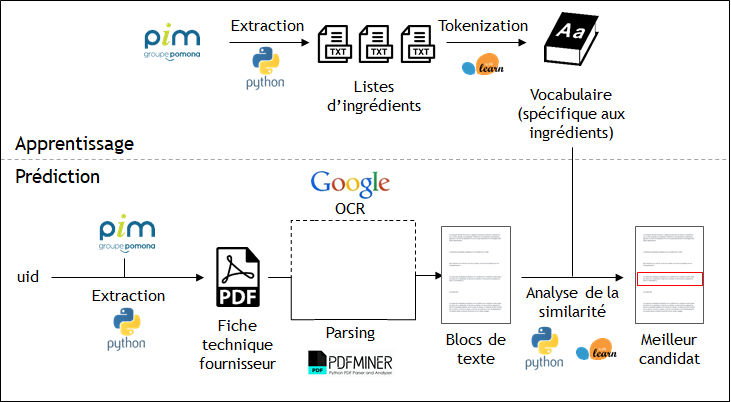
\includegraphics[width=0.9\linewidth]{img/open_model.png}
        \end{center}
        \caption{Schéma de principe du \og modèle ouvert \fg}
        \label{fig:open_model}
    \end{figure}     


        \section{Extraction des données}

        Ne garder que produits d'épicerie et boissons non alcoolisées

        \section{Conversion en blocs de texte}

        On utilise la bibliothèque PDFMiner.six. 
        Elle nous sort un long string qui contient le texte entier du document.
        On applique une \og bête \fg fonction : on splitte ce string quand on observe 2 retours à la lignes consécutifs.
        Le code est présenté en annexe.
        Pour le moment, vu la proportion importante de PDF dont le contenu est extractible

        \section{Train/Test split}

        On fait un split 50/50, on se base sur les uid pour identifier les produits.
        Sur le train set, on récupère les listes d'ingrédients du PIM.

        \section{Entrainement du modèle}

        L'entraînement est basique : on constitue seulement un vocabulaire en utilisant la fonctionnalité mise à disposition dans scikit-learn.

        \section{Calcul de la similarité}

        On calcule la similarité cosinus entre chacun des blocs, et le vocabulaire.
        On prend, systématiquement l'argmax de la similarité qu'on propose comme liste d'ingrédients.

        \section{Illustration des résultats obtenus}
    
        Mettre ici les résultats sur quelques fiches techniques présentées en annexe.
        Spoiler : rien que comme ça, les résultats sont encourageants.

        \section{Pistes d'améliorations identifiées}

        En plus de la mesure de la performance, qui est indispensable avant de pouvoir procéder à des ajustements.
        Pistes identifiées : 
        \begin{itemize}
            \item Faire un découpage du gros texte en blocs plus malin, potentiellement avec des expressions régulières
            \item Faire des \og ngrams de blocs \og, ce qui permettrait de parfois fusionner des blocs qui ont été séparés (car contenaient des retours à la ligne successifs)
            \item Essayer une autre manière de calculer la similarité ?
        \end{itemize}

    \chapter{Utilisation des données manuellement étiquetées}

    Expliciter pourquoi on ne peut pas faire tourner (référence parties précédentes) sur les listes d'ingrédients déjà présentes dans le PIM => soucis de qualité de données source. 
    Si on entraîne sur des données de mauvaise qualité, on aura de mauvais résultats.
    Le code de cette partie est présenté en annexe.    
    Le fonctionnement de ce modèle est présentés à la \reffig{fig:ground_truth_model}.
    
    \begin{figure}[htbp]
        \begin{center}
        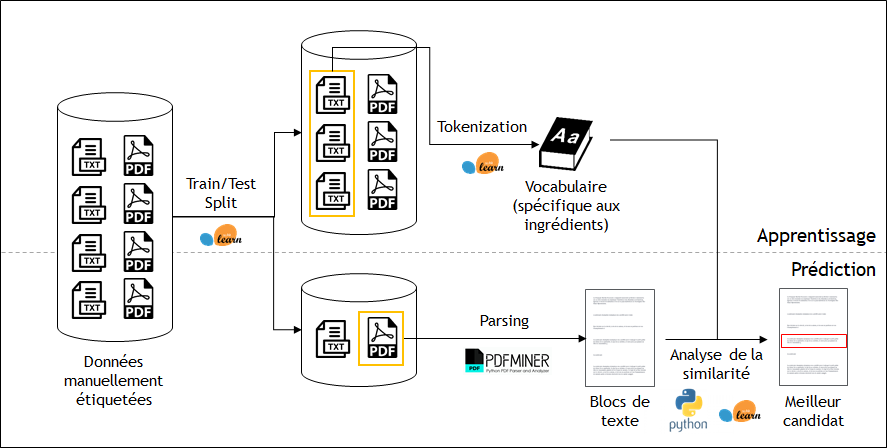
\includegraphics[width=0.9\linewidth]{img/ground_truth_model.png}
        \end{center}
        \caption{Schéma de principe du modèle basé sur les données étiquetées}
        \label{fig:ground_truth_model}
    \end{figure}     


        \section{Chargement des données manuellement étiquetées}

        Un bon vieux read\_csv des familles pour le résultat.
        Les transformations à pipeliner pour les pdf et la constitution des blocs.

        \section{Train/Test split}

        Vu qu'on a moins de données, on fait train = 400 et test = 100.

        \section{Entraînement du modèle}

        On fait tourner de la même manière que sur le modèle dit \og ouvert \fg

        \section{Illustration des prédictions obtenues}

        On illustre ici le résultat.

    \chapter{Mesure de la performance}
    
    Comme vu aux chapitre précédents, il est indispensable de mesurer la performance de nos modèles.
    On le fera sur le modèle se basant sur les données manuellement étiquetées.
    Le principe est présenté à la \reffig{fig:measured_model}.

    \begin{figure}[htbp]
        \begin{center}
        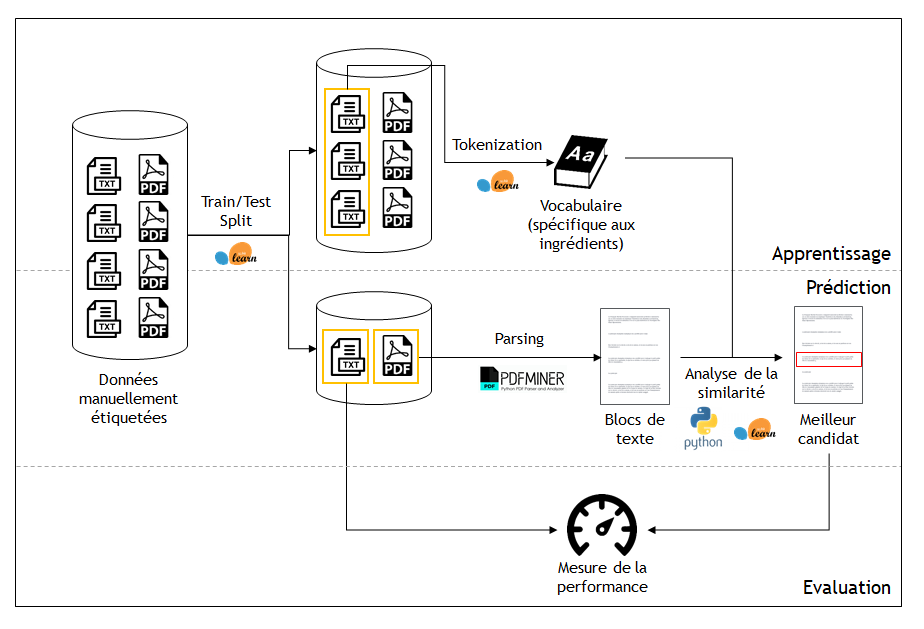
\includegraphics[width=0.9\linewidth]{img/measured_model.png}
        \end{center}
        \caption{Illustration de la méthodologie de mesure de la performance}
        \label{fig:measured_model}
    \end{figure}     

        \section{Précision}
        
        La métrique qui tombe le plus sous le sens est la précision.
        On mesure la proportion de prédictions qui sont égales à la ground truth.

            \subsection{Approche naïve}

            Illustration des résultats. 
            Comme on s'y attend, la précision sans transformation est très sévère.
            En particulier, prise en compte de la casse et des accents.
            La sortie du modèle contient des retours à la ligne à la fin des lignes de texte, là où la ground truth n'en contient pas.

            \subsection{Avec du \og text-postprocessing \fg}
        
            On assouplit un peu les contraintes en effectuant du text processing, à la fois sur la ground truth et les résultats du modèle.
            On tokenize (pour retirer ponctuation, \og blancs \fg), et on retire la casse et les accents pour constituer des textes qui ont plus de chance d'être égaux.
            Ce n'est pas une astuce pour améliorer les résultats, c'est juste que cette manière de mesurer est plus pertinente.
            Illustration des résultats en applicant diverses manières de \og post-processer \fg.

        \section{Fonctions de \og loss \fg spécifiques}

        On peut aussi définir des fonctions de loss, qui permettent d'être plus fin qu'une simple évaluation OK / KO du résultat du modèle.
        On calculera une distance entre le résultat du modèle, et de la ground truth.

            \subsection{Distance de Levenshtein}

            Brève description de chacune de ces distances.

            \subsection{Distance de Dameray-Levenshtein}

            Brève description de chacune de ces distances.
            
            \subsection{Distance de Jaro}
            Brève description de chacune de ces distances.

            \subsection{Distance de Jaro-Wrinkler}
            Brève description de chacune de ces distances.

            \subsection{Métriques non retenues}
            Distance de Hamming

            \subsection{Conclusion sur la métrique à utiliser}
            Une fois que cela aura été fait.


        \section{Cross-validation}
            
        On effectue une cross validation sur le modèle travaillant sur les données manuellement étiquetées.    
        
    \chapter{Transfer learning}
        
        \section{Principe du pré-entraînement}
        
        Expliquer qu'il s'agit d'une approche hybride des 2 modèles précédents
        On effectue une entraînement à la fois sur une partie des listes d'ingrédients du PIM, et sur une partie des données étiquetées.
        On vérifie ensuite, uniquement sur 

        \section{Illustration de l'impact sur la performance}

        Ici, on montre l'impact sur la performance, du fait d'intégrer des listes d'ingrédients.
        On met en abscisse le nombre de listes d'ingrédients qu'on ajoute, et en ordonnée la performance du modèle (avec barre d'erreurs, via cross validation).
        On regarde si l'effet est positif : cela montrera s'il est intéressant d'avoir plus de données.
        On regarde si on observe une saturation : cela montrera si on a déjà suffisamment de données sous formes de listes d'ingrédients dans le PIM, ou bien si ce serait intéressant d'en acquérir plus.

    \chapter{Hyperparameter tuning}
            
    On peut, dans l'optique d'améliorer la performance du modèle, ajuster certains paramètres et d'évaluer l'impact via une grid search.
    On fera tourner sur le modèle avec transfer learning.

        \section{Les paramètres ajustables}

            \subsection{La prise en compte des \og n-grams \fg dans la tokeinzation}

            On peut utiliser les n-grams lors de la tokenisation.

            \subsection{L'application de \og n-grams \fg de blocs}

            Voir si dans la recherche du meilleur candidat, on s'autorise la constitution de \og n-grams \fg de blocs.

            \subsection{L'utilisation d'expressions régulières dans le split des blocs}

            Voir si certaines expressions régulières pour splitter les blocs procurent de meilleurs résultats.

            \subsection{Applications d'autres fonctions de similarité}

            Voir l'impact d'utiliser d'autres manières de calculer la similarité.

            1 - autre chose que la similarité cosinus (fonction du nombre de mots du bloc et de la proportion de mots issus du vocabulaire des ingrédients)

            2 - en appliquant du TF et du TF-IDF

        \section{Application d'une grid search}

        Illustrer ici les résultats d'une grid search ou d'une random search si trop gourmand.